\chapter{Hamilton-Jacobi Theory}
\label{hj}

\section{Hamilton--Jacobi and Madelung Theory}

The Hamilton--Jacobi equation is usually presented as a
nonlinear first-order partial differential equation for a scalar field
$S(q,t)$. However, the fundamental object of classical mechanics is not a
one-point function but the two-point classical action $S(q_0,t_0;q,t)$, defined
as the extremal action between endpoints. The apparent reduction from a
two-point object to a one-point field hides essential geometric and dynamical
information. In particular, the Hamilton--Jacobi formulation is valid only
while the evolving Lagrangian manifold remains a graph over configuration
space. After caustic formation, the velocity field ceases to be globally
representable as a gradient, and the single-valued phase function breaks down.
We analyze the implications of this fact for Hamilton--Jacobi theory, Madelung
hydrodynamics, and stochastic formulations of quantum mechanics.

The Hamilton--Jacobi (HJ) equation occupies a central place in classical
mechanics, geometrical optics, semiclassical quantum mechanics, and stochastic
formulations of quantum theory. It is usually written as
\begin{equation}
\partial_t S + H(q,\nabla S,t)=0,
\label{HJ}
\end{equation}
where $S(q,t)$ is interpreted as a scalar field on configuration spacetime.

This formulation suggests that the theory is an ordinary initial value problem
for a scalar field. However, this interpretation is misleading. The fundamental
classical object is not the one-point function $S(q,t)$ but the two-point
action $S(q_0,t_0;q,t)$, defined as the extremal value of the action functional
between fixed endpoints.

The purpose of this article is to clarify:
\begin{enumerate}
\item how the HJ equation emerges from the two-point action;
\item why the apparent one-point formulation hides essential boundary
    information;
\item why the velocity field ceases to be globally representable as a gradient
    after caustic formation;
\item why Madelung hydrodynamics and related stochastic formulations inherit
    these difficulties.
\end{enumerate}

Consider a classical system with Lagrangian
$L(q,\dot q,t)$.
The Hamilton principal function is defined by
\begin{equation}
S(q_0,t_0;q,t)=\operatorname*{ext}_{q(\tau)}
\int_{t_0}^{t} L(q,\dot q,\tau)\,d\tau,
\label{principal}
\end{equation}
where the extremization is performed over all paths satisfying
$q(t_0)=q_0$, $q(t)=q$.
Thus the classical action is naturally a two-point function on configuration spacetime.

The endpoint variation formulas yield
\begin{equation}
p_i(t)=\frac{\partial S}{\partial q^i},
\qquad
p_i(t_0)=-\frac{\partial S}{\partial q_0^i}.
\label{endpoint}
\end{equation}
Hence the two-point action generates the classical canonical transformation.

Fix the initial endpoint $(q_0,t_0)$ and define
$\mathcal S(q,t):=S(q_0,t_0;q,t)$.
Now vary only the final endpoint. A small variation gives
$\delta S=p_i\,\delta q^i - H\,\delta t$.
Therefore,
$dS = p_i\,dq^i - H\,dt$.
Identifying $p_i=\frac{\partial S}{\partial q^i}$,
one obtains $\frac{\partial S}{\partial t}+
H\left(q,\frac{\partial S}{\partial q},t\right)=0$.
Thus the HJ equation appears only after one endpoint has been frozen.

The reduction from the two-point action to the one-point field hides the
initial endpoint inside the boundary conditions.
Indeed, $S(q,t)=S(q_0,t_0;q,t)$
must satisfy singular initial data:
\begin{equation}
S(q,t_0)=
\begin{cases}
0, & q=q_0,\\
+\infty, & q\neq q_0.
\end{cases}
\end{equation}
Therefore the HJ equation alone does not define the dynamics. The choice of
admissible solutions depends on hidden global information inherited from the
original two-point action.

The geometric meaning of the HJ equation becomes clearer in phase space.
Given a function $S(q,t)$, define $p=\nabla S(q,t)$.
This determines a submanifold $\Lambda_t=\{(q,p):p=\nabla S(q,t)\}\subset T^*Q$.

Initially, one has a graph $\Lambda_0=\{(q,\nabla S_0(q))\}$.
Hamiltonian evolution transports this manifold: $\Lambda_t=\Phi_t(\Lambda_0)$,
where $\Phi_t$ is the Hamiltonian flow.The HJ formulation remains valid only 
while $\Lambda_t$ remains a graph over configuration space.

As the Hamiltonian flow evolves, the Lagrangian manifold generically folds in
phase space. The projection $\pi:\Lambda_t\to Q$ eventually ceases to be
one-to-one. At such points:
\begin{itemize}
\item several classical trajectories reach the same configuration point;
\item several momenta correspond to the same position;
\item the action becomes multivalued;
\item no single velocity field exists.
\end{itemize}
Instead of a single branch $p=\nabla S(q,t)$,
one obtains several branches: $p_1(q,t),\quad p_2(q,t),\quad \dots$
Each branch may locally be represented as a gradient,
$p_i=\nabla S_i$, but globally no single-valued $S(q,t)$ exists.

Suppose particles initially move to the right. A sufficiently strong potential
may reverse some trajectories in finite time. Then at later times a single
position may simultaneously contain:
\begin{itemize}
\item trajectories moving left;
\item trajectories moving right.
\end{itemize}
Therefore the velocity field is no longer single-valued.
This phenomenon is generic and corresponds mathematically to the intersection
of characteristics in first-order PDE theory.

The HJ equation is closely related to Burgers-type equations.
For the free particle Hamiltonian $H=\frac{p^2}{2m}$,
one has $\partial_t S + \frac{(\nabla S)^2}{2m}=0$.
Defining $v=\frac{\nabla S}{m}$, gives $\partial_t v + (v\cdot\nabla)v=0$.
This equation develops shocks through characteristic crossing. Thus the
breakdown of the gradient representation is not exceptional but generic.


\section{Why the Cauchy Problem for the Hamilton--Jacobi Equation\\
Generically Has No Global Solution:\\
Caustics Even in $H=p^2/2m+V(x)$}

We give a self-contained, quantitative account of a fact that is well known to
specialists and routinely surprising on first encounter: the Cauchy
(initial value) problem for the time-dependent Hamilton--Jacobi equation
\[
\partial_t S(x,t) + H\big(x,\partial_x S(x,t)\big) = 0, \qquad S(x,0) = S_0(x),
\]
generically has \emph{no} solution that is smooth and single-valued for all
$t>0$ -- even when $H(x,p) = p^2/2m + V(x)$ is the simplest Hamiltonian in
classical mechanics. We rederive the method of characteristics, reduce the
question of global-in-time smooth solvability to the non-vanishing of a
Jacobian obeying a linear \emph{Jacobi equation}, and show that this
Jacobian generically vanishes in finite time. We then treat, in complete
elementary detail, the free particle and the harmonic oscillator: for the
latter we prove that \emph{every} $C^2$ initial phase $S_0$, however
gentle, produces a singularity by a universal, data-independent time
$t^\ast < \pi/\omega$, and we give the exact closed-form blow-up time. We
explain why this singularity is a geometric \emph{caustic} -- a fold of a
Lagrangian manifold -- rather than a genuine loss of information as in a
shock wave, and we discuss the two standard remedies: the multivalued
semiclassical (WKB/Maslov) continuation, and the single-valued
Crandall--Lions viscosity solution given by a Hopf--Lax-type variational
formula.

\subsection{Introduction}

In a first course, the Hamilton--Jacobi equation (HJE) is usually introduced as
a slightly baroque alternative to Hamilton's equations: separate variables,
find a complete integral, and the trajectories fall out for free. This leaves
the impression that the HJE is an evolution equation on the same footing as the
heat equation or the Schr\"odinger equation, so that prescribing
$S(x,0)=S_0(x)$ ought to determine $S(x,t)$ for all later times, in exact
analogy with how $\psi(x,0)$ determines $\psi(x,t)$ under Schr\"odinger
evolution.

This impression is false, and it fails already for the least exotic Hamiltonian
one can write down,
\begin{equation}
H(x,p) = \frac{p^2}{2m} + V(x),
\label{eq:H}
\end{equation}
with $V$ as smooth and as tame as one likes -- including $V\equiv 0$. The
purpose of this note is to make completely explicit, elementary, and
quantitative the precise sense in which the Cauchy problem for the HJE with
Hamiltonian \eqref{eq:H} cannot, generically, be posed for all time.

We will show the following.
\begin{itemize}
\item[(i)] A local-in-time smooth solution always exists
    (subsection~\ref{sec:characteristics}), constructed by the method of
        characteristics, which reduces the first-order \emph{partial}
        differential equation to Hamilton's \emph{ordinary} differential
        equations.
\item[(ii)] Whether this local solution extends to a given later time $t$ is
    controlled entirely by the non-vanishing of a single scalar quantity
        $J(t,x_0)$ -- the Jacobian of the map ``initial position $\mapsto$
        position at time $t$'' -- which obeys a \emph{linear, second-order}
        ODE, the Jacobi equation (subsection~\ref{sec:jacobi}).
\item[(iii)] For the free particle, $J$ blows down to zero in finite time
    unless the initial phase $S_0$ is convex; ``most'' data are not convex
        (subsection~\ref{sec:free}).
\item[(iv)] For the harmonic oscillator -- arguably \emph{the} most elementary
    confining potential in physics -- $J$ vanishes in finite time for
        \emph{every} choice of $S_0$ whatsoever, with an explicit, universal
        bound on the blow-up time (subsection~\ref{sec:sho}).
\item[(v)] The resulting singularity is not a defect of the method; it is a
    geometric \emph{caustic}, and we explain precisely what it is (a fold
        singularity of a Lagrangian submanifold under projection to
        configuration space) and what it is not (a shock wave, in the sense of
        a scalar conservation law) (subsection~\ref{sec:geometry}).
\item[(vi)] We describe the two standard ways of continuing the solution past
    the singular time -- the multivalued semiclassical construction and the
        single-valued viscosity solution -- and note that both correspond to
        genuinely different, non-classical notions of ``solving'' the HJE
        (subsection~\ref{sec:continuations}).
\end{itemize}

We stress at the outset why this is not a pathology of complicated potentials:
the source of the nonlinearity responsible for all of it is the kinetic term
$p^2/2m$ by itself. As we show in subsection~\ref{sec:free}, the free particle
($V\equiv 0$) already exhibits finite-time breakdown for a generic initial
phase.

\begin{remark}
    Throughout, $S(x,t)$ denotes Hamilton's \emph{principal function}, the solution
    of the time-dependent HJE $\partial_tS + H(x,\partial_xS)=0$. This should
    not be confused with Hamilton's \emph{characteristic function} $W(x,E)$,
    which solves the time-independent equation $H(x,\partial_xW)=E$ and is used
    for separable, energy-conserving problems; the characteristic function is
    unproblematic to define (it is just a line integral of
    $p(x,E)=\pm\sqrt{2m(E-V(x))}$) and is not the subject of this paper. It is
    $S(x,t)$, the \emph{generator of the time-$t$ flow as a canonical
    transformation}, whose Cauchy problem is generically ill-posed for all
    time.
\end{remark}

\subsection{The Hamilton--Jacobi Cauchy problem}
\label{sec:setup}

Fix a mass $m>0$ and a potential $V\in C^k(\mathbb{R})$, $k\ge 2$, and let $H$
be as in \eqref{eq:H}. The Cauchy problem under discussion is: given 
$S_0 \in C^k(\mathbb{R})$, 
find $S\in C^1(\mathbb{R}\times[0,T))$, for as large a $T$ as
possible, solving
\begin{equation}
\partial_t S(x,t) + \frac{1}{2m}\big(\partial_x S(x,t)\big)^2 + V(x) = 0, \qquad S(x,0)=S_0(x).
\label{eq:HJE}
\end{equation}

Recall the mechanical meaning of $S$: if $S$ solves \eqref{eq:HJE}, then the
vector field $p(x,t):=\partial_xS(x,t)$ is a \emph{momentum field} -- at each
point $x$ and time $t$, it prescribes the momentum of the classical trajectory
passing through $x$ at time $t$ -- and $S(x,t)$ equals the classical action
accumulated along that trajectory since $t=0$,
\begin{equation}
S(x,t) = S_0(x_0) + \int_0^t L\big(x(\tau),\dot x(\tau)\big)\,d\tau, \qquad L(x,\dot x)=\tfrac12 m\dot x^2 - V(x),
\label{eq:action}
\end{equation}
where $x(\cdot)$ is the classical trajectory with $x(0)=x_0$ and $x(t)=x$.
Equation \eqref{eq:action} is not an assumption; it is a theorem, proved in
subsection~\ref{sec:characteristics} below.

The question we address is exactly: for which $T$ does there exist a single
$C^1$ function on $\mathbb{R}\times[0,T)$ (or on some fixed spatial domain of
interest, times $[0,T)$) satisfying \eqref{eq:HJE} pointwise? We will see that
the honest answer, for essentially every choice of $V$ and $S_0$, is:
\emph{only for $T$ up to some finite $t^\ast$}, no matter how smooth $V$ and
$S_0$ are.

\subsection{Characteristics: the PDE becomes an ODE}
\label{sec:characteristics}

\begin{proposition}[Characteristics of the HJE]
\label{prop:characteristics}
Suppose $S\in C^2(\mathbb{R}\times[0,T))$ solves \eqref{eq:HJE}. Fix
    $x_0\in\mathbb{R}$ and let $x(\cdot)$ solve the ordinary differential
    equation
\[
\dot x(t) = \partial_pH\big(x(t),\partial_xS(x(t),t)\big) =
    \frac{1}{m}\partial_xS(x(t),t), \qquad x(0)=x_0,
\]
for as long as this makes sense. Set $p(t):=\partial_xS(x(t),t)$ 
    and $\sigma(t):=S(x(t),t)$. Then
\begin{equation}
\dot x = \frac{p}{m}, \qquad \dot p = -V'(x), 
    \qquad \dot\sigma = p\dot x - H(x,p) = L(x,\dot x).
\label{eq:hameqs}
\end{equation}
That is, $(x(t),p(t))$ is a solution of Hamilton's equations, and $\sigma$ is
    the classical action accumulated along it.
\end{proposition}

\begin{proof}
Differentiate the defining relation for $p$ along the curve:
\[
\dot p = \frac{d}{dt}\,\partial_xS(x(t),t) = \partial_t\partial_xS +
    \dot x\,\partial_x^2 S.
\]
Differentiate the PDE \eqref{eq:HJE} itself with respect to $x$:
\[
\partial_x\partial_tS + V'(x) + \frac{1}{m}\partial_xS\,\partial_x^2S = 0
\quad\Longrightarrow\quad
\partial_t\partial_xS = -V'(x) - \dot x\,\partial_x^2S,
\]
where we used $\dot x = \frac1m\partial_xS(x(t),t)=\frac1m p$. Substituting,
\[
\dot p = \big(-V'(x)-\dot x\,\partial_x^2S\big) + \dot x\,\partial_x^2S = -V'(x),
\]
which is the second equation in \eqref{eq:hameqs}. Finally,
\[
\dot\sigma = \frac{d}{dt}S(x(t),t) = \partial_tS + \dot x\,\partial_xS = -H(x,p) + \dot x\,p = p\dot x - H(x,p),
\]
using \eqref{eq:HJE} for $\partial_tS$. Since $H(x,p)=p^2/2m+V(x)$ is the Legendre transform of $L(x,\dot x)=\tfrac12m\dot x^2-V(x)$ with $p=m\dot x$, and $\dot x=p/m$ by construction, we have $p\dot x-H(x,p)=L(x,\dot x)$ exactly.
\end{proof}

Proposition~\ref{prop:characteristics} converts the search for $S$ into the
elementary task of solving Hamilton's equations, an autonomous system of ODEs
with smooth (as smooth as $V$) right-hand side, hence with a smooth, locally
unique flow. Denote by $(x(t;x_0),p(t;x_0))$ the solution with
\[
x(0;x_0)=x_0, \qquad p(0;x_0)=S_0'(x_0),
\]
and define the \textbf{stretching factor}
\begin{equation}
J(t,x_0) := \frac{\partial x}{\partial x_0}(t;x_0).
\label{eq:Jdef}
\end{equation}
By construction $J(0,x_0)=1$ for every $x_0$.

\begin{theorem}[Local solvability, and its limit]
\label{thm:local}
Let $V,S_0\in C^k(\mathbb{R})$, $k\ge 2$. Fix $x_0$, and let
\begin{equation}
t^\ast(x_0) := \sup\{\,T>0 : J(t,x_0)\ne 0 \text{ for all } t\in[0,T)\,\} \ \in (0,\infty].
\label{eq:tstar}
\end{equation}
Then for every $T<t^\ast(x_0)$ there is an interval $I\ni x_0$ and a
    neighborhood of $\{x(t;x_0): t\in[0,T]\}$ on which $x_0\mapsto x(t;x_0)$
    is, for each fixed $t\le T$, a $C^{k-1}$ diffeomorphism from $I$ onto its
    image; writing $x_0(x,t)$ for its inverse, the function
\[
S(x,t) := S_0\big(x_0(x,t)\big) + \int_0^t L\Big(x\big(\tau;x_0(x,t)\big),
    \dot x\big(\tau;x_0(x,t)\big)\Big)\,d\tau
\]
is the unique $C^1$ solution of \eqref{eq:HJE} on that neighborhood, for
    $t\in[0,T]$. Conversely, no single-valued $C^1$ function can solve
    \eqref{eq:HJE} in any neighborhood of
    $\big(x(t^\ast(x_0);x_0),t^\ast(x_0)\big)$ extending past $t=t^\ast(x_0)$,
    if $x_0\mapsto x(t;x_0)$ fails to be injective near $x_0$ for $t$ slightly
    larger than $t^\ast(x_0)$ -- which is the generic situation.
\end{theorem}

\begin{proof}[Proof sketch]
Existence for $t<t^\ast(x_0)$: since $J(0,x_0)=1\ne0$ and $J$ is continuous,
    $J\ne0$ on $[0,T]$ for $T<t^\ast(x_0)$; by the inverse function theorem,
    $x_0\mapsto x(t;x_0)$ is then a local diffeomorphism, uniformly for
    $t\in[0,T]$, on some interval $I$. That the resulting $S(x,t)$ solves
    \eqref{eq:HJE} is a direct (if slightly tedious) computation using
    Proposition~\ref{prop:characteristics} in reverse, and is the classical
    content of the method of characteristics for first-order PDEs; see
    Courant--Hilbert \cite{CourantHilbert} or Evans \cite{Evans}, \S3.2--3.3.

Uniqueness, and the impossibility of continuation: if $\tilde S$ is \emph{any}
    $C^1$ solution of \eqref{eq:HJE} near a point $(x,t)$, set $\tilde
    p(x,t):=\partial_x\tilde S(x,t)$ and let $\tilde x(\cdot)$ solve
    $\dot{\tilde x}=\tilde p(\tilde x,\cdot)/m$ through $(x,t)$. Running
    Proposition~\ref{prop:characteristics}'s argument backward in time shows
    $(\tilde x(\cdot),\tilde p(\tilde x(\cdot),\cdot))$ satisfies Hamilton's
    equations; by uniqueness of solutions of ODEs with Lipschitz right-hand
    side, this trajectory must coincide with $(x(\cdot;x_0),p(\cdot;x_0))$ for
    the appropriate $x_0$. Hence \emph{every} $C^1$ solution, wherever defined,
    must agree with the characteristic construction. If, at time
    $t>t^\ast(x_0)$, two distinct characteristics $x_0\ne x_0'$ satisfy
    $x(t;x_0)=x(t;x_0')=x$, then any $C^1$ solution would be forced to satisfy
    $\partial_x\tilde S(x,t) = p(t;x_0)$ \emph{and} $\partial_x\tilde
    S(x,t)=p(t;x_0')$ simultaneously; if $p(t;x_0)\ne p(t;x_0')$ (the generic
    case at a simple fold), this is a contradiction, so no such $\tilde S$
    exists.
\end{proof}

Theorem~\ref{thm:local} reduces everything to the study of $J(t,x_0)$, i.e., to
a linear second-order ODE, which we derive next.

\subsection{The Jacobi equation and the breakdown criterion}
\label{sec:jacobi}

Differentiate Hamilton's equations \eqref{eq:hameqs} with respect to the label
$x_0$. Writing $J=\partial_{x_0}x$ and $K=\partial_{x_0}p$,
\[
\dot J = \frac{1}{m}K, \qquad \dot K = -V''\big(x(t;x_0)\big)\,J,
\]
and hence
\begin{equation}
\ddot J(t,x_0) + \frac{1}{m}V''\big(x(t;x_0)\big)\,J(t,x_0) = 0, \qquad J(0,x_0)=1, \quad \dot J(0,x_0) = \frac{S_0''(x_0)}{m}.
\label{eq:jacobi}
\end{equation}
This is precisely the \emph{Jacobi equation} (Jacobi accessory equation) of the
classical calculus of variations, governing the second variation of the action
along the extremal $x(\cdot;x_0)$; see Arnold \cite{Arnold}, \S22--23, or
Milnor \cite{Milnor}, \S15. A zero of $J$ is, by definition, a
\textbf{conjugate point} along the trajectory. So Theorem~\ref{thm:local} says:

\begin{center}
\emph{the smooth HJE solution breaks down at exactly the first conjugate point.}
\end{center}

This is not a coincidence but the same fact seen from two sides: a conjugate
point is exactly the point where the trajectory $x(\cdot;x_0)$ stops being even
a local minimizer of the action (Jacobi's necessary condition), and it is
exactly the point where the family of nearby trajectories, which the generating
function $S$ is supposed to organize into a single-valued momentum field,
starts to overlap.

\begin{remark}
Up to normalization, $J(t,x_0)^{-1}$ is (the one-dimensional case of) the Van
    Vleck--Morette determinant that controls the amplitude of the semiclassical
    (WKB) approximation to the quantum propagator. Its vanishing is precisely
    the condition under which the leading-order WKB amplitude diverges,
    signalling the breakdown of the naive semiclassical approximation and the
    need for Airy-function (uniform) corrections near the caustic; see
    Maslov--Fedoriuk \cite{MaslovFedoriuk} and Guillemin--Sternberg
    \cite{GuilleminSternberg}.
\end{remark}

We now solve \eqref{eq:jacobi} explicitly for the two simplest potentials there are.

\subsection{Two boring examples}
\label{sec:examples}

\subsubsection{The free particle}
\label{sec:free}

Take $V\equiv0$. Then $V''\equiv0$ and \eqref{eq:jacobi} integrates trivially:
\begin{equation}
J(t,x_0) = 1 + \frac{S_0''(x_0)}{m}\,t.
\label{eq:Jfree}
\end{equation}

\begin{proposition}
\label{prop:free}
For the free particle, the classical HJE solution starting from $x_0$ exists
    for all $t>0$ if and only if $S_0''(x_0)\ge 0$. If $S_0''(x_0)<0$, it
    breaks down at the finite time
\[
t^\ast(x_0) = -\frac{m}{S_0''(x_0)}.
\]
\end{proposition}

The condition $S_0''\ge0$ everywhere means $S_0$ is convex: the initial
momentum field $p_0(x)=S_0'(x)$ is non-decreasing, so nearby particles are, at
worst, drifting apart or moving in parallel -- never converging. This is a very
restrictive condition (violated, for instance, on an open dense set of $C^2$
functions in any reasonable topology): the mere presence of one convergent
region in the initial data destroys global existence.

\begin{example}[A lens]
Take $S_0(x) = -\dfrac{m}{2\tau}x^2$ for some $\tau>0$, i.e., an initial
    momentum field $p_0(x)=-\frac{m}{\tau}x$ pointing uniformly toward the
    origin -- literally the phase profile of a converging lens. Every
    characteristic is a straight line,
\[
x(t;x_0) = x_0\Big(1-\frac{t}{\tau}\Big),
\]
and \emph{all of them meet at the single point $x=0$ at time $t=\tau$}: a
    perfect focus, formed instantly out of the most boring possible dynamics
    (free motion) acting on smooth, everywhere-defined data. See
    Figure~\ref{fig:focus}.
\end{example}

\begin{figure}[h]
\centering
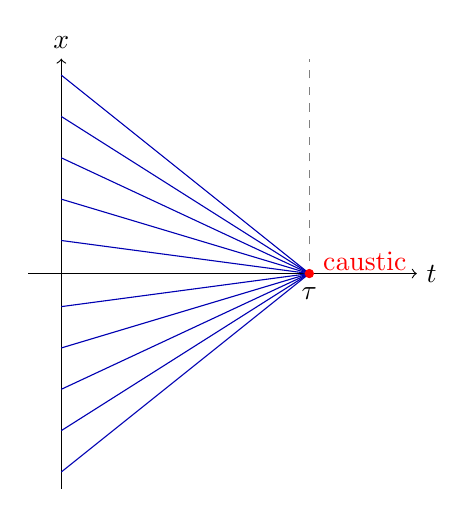
\begin{tikzpicture}[scale=1.05]
\draw[->] (-0.4,0) -- (4.3,0) node[right] {$t$};
\draw[->] (0,-2.6) -- (0,2.6) node[above] {$x$};
\draw[dashed,gray] (3,-0.05) -- (3,2.6);
\node[below] at (3,-0.05) {$\tau$};
\foreach \xa in {-2.4,-1.9,-1.4,-0.9,-0.4,0.4,0.9,1.4,1.9,2.4}{
  \draw[thin,blue!70!black] (0,\xa) -- (3,0);
}
\filldraw[red] (3,0) circle (1.4pt);
\node[right,red] at (3.05,0.15) {caustic};
\end{tikzpicture}
\caption{Characteristics $x(t;x_0)=x_0(1-t/\tau)$ of the free particle with
    converging initial phase $S_0(x)=-\frac{m}{2\tau}x^2$. Every trajectory,
    however far from the origin it starts, reaches $x=0$ at the same instant
    $t=\tau$: a caustic forms in finite time even though $V\equiv0$.}
\label{fig:focus}
\end{figure}

\subsubsection{The harmonic oscillator}
\label{sec:sho}

Take $V(x)=\tfrac12 m\omega^2x^2$, so $V''\equiv m\omega^2$ is constant, and
\eqref{eq:jacobi} becomes the harmonic-oscillator equation itself,
\[
\ddot J + \omega^2 J = 0, \qquad J(0,x_0)=1,\quad \dot J(0,x_0)=\frac{S_0''(x_0)}{m},
\]
with exact solution
\begin{equation}
J(t,x_0) = \cos\omega t + \frac{S_0''(x_0)}{m\omega}\sin\omega t.
\label{eq:Jsho}
\end{equation}

\begin{theorem}[Universal breakdown]
\label{thm:sho}
For the harmonic oscillator, for \emph{every} $S_0\in C^2(\mathbb{R})$ and
    \emph{every} $x_0\in\mathbb{R}$, the classical HJE solution starting from
    $x_0$ breaks down at the finite time
\begin{equation}
t^\ast(x_0) = \frac{1}{\omega}\left[\frac{\pi}{2} + \arctan\!\left(\frac{S_0''(x_0)}{m\omega}\right)\right] \ \in\ \Big(0,\ \frac{\pi}{\omega}\Big).
\label{eq:tstarsho}
\end{equation}
In particular $t^\ast(x_0) < \pi/\omega$ uniformly in $x_0$ and in $S_0$: no choice of smooth initial phase, however gentle, avoids a caustic within one half-period of the oscillator.
\end{theorem}

\begin{proof}
Write $A=1$, $B=S_0''(x_0)/(m\omega)$, so $J(t,x_0)=A\cos\omega t+B\sin\omega t
    = R\cos(\omega t-\phi)$ with $R=\sqrt{A^2+B^2}>0$ and
    $\phi=\arctan(B/A)=\arctan B\in(-\tfrac\pi2,\tfrac\pi2)$ (the branch is
    fixed by $A=1>0$). The zeros of $J$ are at $\omega t-\phi=\tfrac\pi2+k\pi$,
    $k\in\mathbb Z$, i.e. $t=(\phi+\tfrac\pi2+k\pi)/\omega$. Since
    $\phi\in(-\tfrac\pi2,\tfrac\pi2)$, the value at $k=0$ lies in
    $(0,\pi/\omega)$ and is manifestly the smallest positive root (the $k=-1$
    root is negative). This proves \eqref{eq:tstarsho}.
\end{proof}

Sanity checks on \eqref{eq:tstarsho}: if $S_0''(x_0)=0$ (locally ``flat''
data), $t^\ast=\pi/(2\omega)$, a quarter period. As $S_0''(x_0)\to+\infty$
(strongly diverging data), $t^\ast\to\pi/\omega$ but never reaches it. As
$S_0''(x_0)\to-\infty$ (strongly focusing data), $t^\ast\to0^+$: an
already-converging beam focuses almost instantly, exactly as one would guess.
What Theorem~\ref{thm:sho} adds is that \emph{even the most favorable, most
divergent possible data cannot postpone the caustic past $t=\pi/\omega$}. This
finite, data-independent interval between conjugate points is a classical fact
about the harmonic oscillator (Arnold \cite{Arnold}, \S23) and is the
mechanical origin of the Maslov index increasing by one unit every half-period
in the semiclassical (Bohr--Sommerfeld--Maslov) quantization of the oscillator.

\subsubsection{General uniformly convex potentials}

Theorem~\ref{thm:sho} is not special to the exactly quadratic potential; it is
the model case of a much more general comparison principle.

\begin{theorem}
\label{thm:sturm}
Suppose $V\in C^2(\mathbb{R})$ satisfies $V''(x)\ge m\omega^2$ for all
    $x\in\mathbb{R}$, for some $\omega>0$. Then for every $S_0\in
    C^2(\mathbb{R})$ and every $x_0\in\mathbb{R}$,
\[
t^\ast(x_0) < \frac{\pi}{\omega}.
\]
\end{theorem}

\begin{proof}
Along the trajectory, $q(t):=V''\big(x(t;x_0)\big)/m \ge \omega^2$ for all $t$,
    so $J$ solves $\ddot J + q(t)J=0$ with $J(0,x_0)=1\ne0$. Let
    $y(t)=\sin\omega t$, which solves $\ddot y+\omega^2y=0$ and has consecutive
    zeros at $t=0$ and $t=\pi/\omega$, with $y\ne0$ in between. By the Sturm
    comparison theorem (see, e.g., Coddington--Levinson
    \cite{CoddingtonLevinson}, Ch.~8) applied to $\ddot J+qJ=0$ against $\ddot
    y+\omega^2y=0$ with $q\ge\omega^2$, $J$ must vanish somewhere in
    $(0,\pi/\omega)$ unless $J$ is a constant multiple of $y$ -- impossible
    here since $J(0,x_0)=1\ne 0=y(0)$.
\end{proof}

\begin{remark}
Theorem~\ref{thm:sturm} is the exact one-dimensional mechanical analogue of the
    Rauch comparison theorem in Riemannian geometry (see do Carmo
    \cite{doCarmo}), in which $V''$ plays the role of subsectional curvature: a
    lower bound on curvature (here, on the ``restoring strength'' of the
    potential) forces conjugate points to appear within a bounded distance --
    the mechanical cousin of the Bonnet--Myers theorem. Convexity of $V$ is
    what does the damage; potentials that are flat or concave ($V''\le0$)
    behave more like the free particle of subsection~\ref{sec:free}, where global
    existence is possible but only for a non-generic (convex) subset of initial
    data.
\end{remark}

\subsection{What the singularity actually is: caustics, not shocks}
\label{sec:geometry}

It is tempting, on seeing \eqref{eq:jacobi} blow down to zero, to think of this
as a shock wave forming out of smooth data, as in Burgers' equation. The
analogy is real but must be handled carefully, because taken too literally it
suggests the wrong physical resolution.

Differentiating \eqref{eq:HJE} once in $x$ and writing $p=\partial_xS$ gives the momentum-field equation
\begin{equation}
\partial_tp + \frac{1}{m}\,p\,\partial_xp = -V'(x).
\label{eq:burgers}
\end{equation}
For $V\equiv0$ this is exactly the inviscid Burgers equation for $u=p/m$, whose
characteristics are the same straight lines drawn in Figure~\ref{fig:focus}. So
far the analogy is exact. But there is a crucial difference in what the
crossing of characteristics \emph{means}.

Consider the full phase-space curve
\[
\Lambda_t := \big\{(x(t;x_0),p(t;x_0)) : x_0\in\mathbb{R}\big\} \subset \mathbb{R}^2.
\]
Because the Hamiltonian flow generated by \eqref{eq:H} is, for the potentials
considered here, a complete flow of smooth diffeomorphisms of the phase plane
for all $t\in\mathbb{R}$, the curve $\Lambda_t$ is perfectly smooth for
\emph{every} $t$ -- nothing in phase space ever collides, merges, or loses
information: this is just Liouville's theorem together with uniqueness of
solutions of Hamilton's equations. What happens at $t=t^\ast(x_0)$ is entirely
a statement about the \emph{projection}
\[
\pi:\Lambda_t\to\mathbb{R}_x, \qquad (x,p)\mapsto x,
\]
whose derivative along $\Lambda_t$ at the point labelled by $x_0$ is exactly
$J(t,x_0)$. At $t=t^\ast(x_0)$, $\pi$ develops a critical point: $\Lambda_t$ is
momentarily tangent to the fibre direction there. This is a \emph{fold}, in the
sense of Whitney and Thom's theory of singularities of smooth maps (see Arnold
\cite{ArnoldCatastrophe} for an accessible account); immediately afterward,
$\pi$ is locally two-to-one, and two distinct sheets of $\Lambda_t$ -- two
distinct momenta -- sit over the same $x$. This is precisely a \emph{caustic}
in the sense of geometric optics: the bright curve on the floor of a swimming
pool, the cusp of a rainbow, the focal point of a lens in
Figure~\ref{fig:focus}. Rays (here, classical trajectories) do not disappear or
merge at a caustic; they simply cross, and go on to occupy the same point in
configuration space while carrying different momenta.

This is fundamentally different from a genuine shock in a scalar conservation
law, such as \eqref{eq:burgers} interpreted on its own as an evolution equation
for $p$ with, say, an entropy condition imposed to select a unique
discontinuous weak solution. That construction is appropriate for a dissipative
medium -- pressureless, sticky ``dust'' in which colliding particles merge and
information is genuinely lost, enforcing the Rankine--Hugoniot / Oleinik
entropy condition. It is not appropriate for the actual, collisionless
mechanical system \eqref{eq:hameqs} describes, in which trajectories pass
through one another. The two constructions coincide as pieces of formal
mathematics (the Lax--Oleinik entropy solution of \eqref{eq:burgers} is
literally $\partial_x$ of the Crandall--Lions viscosity solution of
\eqref{eq:HJE}, discussed in subsection~\ref{sec:continuations}), but they answer
different physical questions. This distinction is exactly the one drawn, in a
cosmological setting, between the ``adhesion approximation'' (dust that sticks
upon crossing, described by the entropy solution) and the true collisionless
dynamics of the Zel'dovich approximation to large-scale structure formation, in
which multiple streams of matter coexist after crossing and form a genuinely
multivalued velocity field; see Zel'dovich \cite{Zeldovich}.

\subsection{Continuations past \texorpdfstring{$t^\ast$}{t*}}
\label{sec:continuations}

Given that no single-valued classical solution survives past the first caustic,
there are two standard, and genuinely different, ways to say something about
$t>t^\ast$.

\subsubsection{Multivalued continuation: the semiclassical picture}

The honest object that continues smoothly through the caustic is not $S(x,t)$
but the Lagrangian curve $\Lambda_t$ itself, which remains smooth for all time.
Near a fold, $\Lambda_t$ is more naturally parametrized by $p$ (or by
arclength) than by $x$, and the correct statement of ``the solution'' becomes:
locally, finitely many smooth branches $S_1(x,t),S_2(x,t),\dots$, one for each
sheet of $\Lambda_t$ lying over $x$.

This is exactly what happens, one order more precisely, in the semiclassical
(WKB) approximation to the Schr\"odinger equation. Substituting
$\psi(x,t)\approx A(x,t)e^{iS(x,t)/\hbar}$ into the Schr\"odinger equation and
expanding in powers of $\hbar$ produces \eqref{eq:HJE} at leading order and a
transport equation for $A$ at the next order, with $A\propto |J|^{-1/2}$; the
WKB amplitude literally diverges at the caustic, exactly where $J=0$. The
correct continuation is a coherent sum over the branches, each carrying an
extra phase $-i\pi\mu_j/2$ where $\mu_j$ (the Maslov index of that branch)
counts the conjugate points crossed so far; near the caustic itself, this
asymptotic sum must be replaced by an Airy-function uniform approximation. See
Maslov--Fedoriuk \cite{MaslovFedoriuk}, Guillemin--Sternberg
\cite{GuilleminSternberg}, and Berry--Upstill \cite{BerryUpstill} for the full
theory of these ``catastrophe optics'' corrections.

\subsubsection{Single-valued continuation: viscosity solutions}
\label{sec:viscosity}

Alternatively, one can insist on a single-valued function of $(x,t)$ defined
for \emph{all} time, at the cost of giving up smoothness. Define
\begin{equation}
S(x,t) \ :=\ \inf\Big\{\, S_0\big(\gamma(0)\big) + \int_0^tL\big(\gamma(\tau),\dot\gamma(\tau)\big)\,d\tau \ :\ \gamma \text{ absolutely continuous}, \ \gamma(t)=x \,\Big\},
\label{eq:hopflax}
\end{equation}
minimizing the total ``cost'' over \emph{all} paths ending at $x$ at time $t$,
with free initial point weighted by $S_0$. Because $L(x,\dot x)=\tfrac12m\dot
x^2-V(x)$ is strictly convex and superlinear in $\dot x$, this variational
problem is well posed for reasonable $V$ (e.g. bounded below, as for both
examples above), and \eqref{eq:hopflax} defines the unique \emph{viscosity
solution} of the Cauchy problem \eqref{eq:HJE}, in the sense of Crandall and
Lions \cite{CrandallLions}, for all $t\ge 0$ -- see Evans \cite{Evans}, Ch.~10,
or Fathi \cite{Fathi} for the Lagrangian (weak KAM) formulation of
\eqref{eq:hopflax}. (When $V$ is constant, minimizing paths are straight lines
and \eqref{eq:hopflax} reduces to the familiar Hopf--Lax formula.)

This $S$ agrees with the classical smooth solution of Theorem~\ref{thm:local}
for $t<t^\ast$, but for $t\ge t^\ast$ it typically develops a genuine kink -- a
jump in $\partial_xS$ -- exactly where two or more competing paths tie for the
minimum in \eqref{eq:hopflax}. In other words, \eqref{eq:hopflax} \emph{can} be
solved globally in time, but only by (i) discarding all but the single
\emph{minimal-action} branch at each point -- throwing away the very
trajectories whose mutual interference is physically encoded in the multivalued
WKB picture -- and (ii) accepting a solution that is merely Lipschitz, not
$C^1$, and therefore no longer ``the'' generating function of a canonical
transformation in the sense classical mechanics requires. This is the precise,
sharp form of the opening claim: a global solution in the classical
(single-sheeted, $C^1$) sense generically does not exist, and neither of the
two standard substitutes -- the multivalued semiclassical one or the
single-valued viscosity one -- is that classical solution; each recovers it
only for $t<t^\ast$ and replaces it with something structurally different
afterward.

\subsection{Discussion and conclusion}

The point of working out the free particle and the harmonic oscillator in such
elementary detail is to make it impossible to blame the phenomenon on some
contrived feature of $V(x)$. The free particle shows that the quadratic kinetic
term \emph{by itself} is enough to produce finite-time breakdown, for any
initial phase with a single region of concavity. The harmonic oscillator shows
that once any amount of convexity is added to $V$, breakdown becomes not merely
generic but \emph{unconditional}: literally no choice of $C^2$ initial data
survives past $t=\pi/\omega$. Between these two examples lies essentially every
problem discussed in an introductory mechanics course.

It is worth closing with the observation that this whole difficulty is a purely
classical artifact, absent from the parent theory. The HJE \eqref{eq:HJE} is
recovered from the Schr\"odinger equation for $\psi=Ae^{iS/\hbar}$ at leading
order in $\hbar$; the linear Schr\"odinger equation itself has a perfectly
well-posed, globally-in-time, unitary Cauchy problem for the same $H$. The
finite-time singularity of the classical theory is not a sign that something is
wrong with mechanics; it is a sign that the eikonal (leading-order,
$\hbar\to0$) approximation to a wave equation must generically develop
caustics, exactly as it does in ordinary geometric optics, and that resolving
them -- whether by keeping all interfering branches (semiclassical
continuation) or by passing to the variational, minimal-action solution
(viscosity continuation) -- requires input beyond the bare Cauchy data $S_0$.
What cannot be done, for essentially any $V$ and essentially any $S_0$, is what
a first encounter with the equation suggests should be routine: solve the
Cauchy problem once, classically, and be done with it for all time.


\section{Why the Initial-Value Problem Makes No Sense for the Hamilton--Jacobi Equation}

Hamilton's canonical equations $\dot q=\partial H/\partial p$, $\dot
p=-\partial H/\partial q$ admit a genuine initial-value problem: fix
$(q_0,p_0)\in T^*Q$ at a time $t_0$ and the future is determined, by the
ordinary Picard--Lindel\"of theorem. The Hamilton--Jacobi equation $\partial
S/\partial t + H(q,\partial S/\partial q,t)=0$ is often introduced as though it
carried an analogous initial-value problem, and it is tempting---since the
equation is first order in $t$---to imagine that fixing $S$, or $S$ together
with $\partial S/\partial q$, at a single point $(q_0,t_0)$ should play the
same role for the field $S(q,t)$ that fixing $(q_0,p_0)$ plays for a single
trajectory. This is false, and provably so. We exhibit an explicit pair of
solutions of the free-particle Hamilton--Jacobi equation that agree in value
and gradient at one spacetime point but disagree everywhere else, showing that
pointwise data of this kind pins down nothing beyond that single point. We then
identify the structural reason: the characteristics of the Hamilton--Jacobi
equation are exactly Hamilton's canonical equations, so a single dynamical
trajectory is exactly a characteristic curve of the PDE, and the general theory
of first-order PDE says that data prescribed along a characteristic is never
free Cauchy data---it is either automatically consistent with the equation, and
so carries no information transverse to the curve, or it is inconsistent with
the equation altogether. The only notion of ``initial data'' that is well posed
for the Hamilton--Jacobi equation is Cauchy data on an entire noncharacteristic
hypersurface: a full function $S_0(q)$, not a point and not a curve. We close
by explaining, via the correspondence between such data and Lagrangian
submanifolds of $T^*Q$, why this correct notion is doing something conceptually
different from---and much richer than---what Hamilton's own initial-value
problem does, and why even it is only locally well posed in time.

\subsection{Introduction}
\label{intro}

Two objects sit side by side in every treatment of classical mechanics. The
first is Hamilton's canonical system,
\begin{equation}
\label{Ham}
\dot q^i = \frac{\partial H}{\partial p_i}, \qquad \dot p_i = -\frac{\partial H}{\partial q^i}, \qquad i=1,\dots,n,
\end{equation}
a system of $2n$ ordinary differential equations on phase space $T^*Q$. The
second is the Hamilton--Jacobi equation,
\begin{equation}
\label{HJ}
\frac{\partial S}{\partial t} + H\Big(q,\frac{\partial S}{\partial q},t\Big) = 0,
\end{equation}
a single partial differential equation for a scalar function $S(q,t)$.
Textbooks derive~\eqref{HJ} from~\eqref{Ham} (or vice versa) in a few lines,
and the two are indeed equivalent in a precise sense made rigorous by Jacobi's
theorem on complete integrals. That equivalence, together with the fact
that~\eqref{HJ} is written as ``$\partial S/\partial t$ equals something,''
first order in $t$ just as~\eqref{Ham} is first order in $t$, invites a
natural-seeming question: what is the initial-value problem for the
Hamilton--Jacobi equation? If one can fix $(q_0,p_0)$ at $t_0$ and thereby
determine the entire future of~\eqref{Ham}, should one not be able to fix
$S(q_0,t_0)$---perhaps together with $\partial S/\partial q$ there, so as to
match the amount of data $(q_0,p_0)$ supplies---and thereby determine the
entire future of~\eqref{HJ}?

The answer is no, and the purpose of this paper is to explain exactly why, in
enough detail that the failure is not merely asserted but demonstrated. The
short version is a type mismatch. The unknown in~\eqref{Ham} at a given time is
a point of $T^*Q$: $2n$ real numbers. The unknown in~\eqref{HJ} at a given time
is a function of $q$ on all of $Q$: an element of an infinite-dimensional
space. An equation that is ``first order in $t$'' for an object of the second
kind does not, in general, admit initial data at a point, for exactly the same
reason that no evolution equation for a field---the heat equation, the wave
equation, ordinary fluid dynamics---admits initial data at a point. What is
special about the Hamilton--Jacobi equation is not that this general PDE fact
holds, but \emph{why} it holds in a way that is unusually easy to state
precisely: the characteristics of~\eqref{HJ} are exactly the trajectories
of~\eqref{Ham}, so the single most natural-looking candidate for ``initial data
along a trajectory'' turns out to be data prescribed along a characteristic
curve of the PDE---which the general theory of first-order PDE identifies as
precisely the case in which prescribed data carries no genuine information at
all.

subsection~\ref{two-objects} separates two objects that share the name
``action'' and are routinely conflated. subsection~\ref{ham-ivp} recalls
why~\eqref{Ham} has a genuine, finite-dimensional initial-value problem.
subsection~\ref{counterexample} gives an explicit counterexample: two solutions
of the same Hamilton--Jacobi equation, agreeing in value and gradient at one
point, disagreeing everywhere else. subsection~\ref{characteristics} supplies
the structural explanation, via the method of characteristics, for why this had
to happen, and sharpens it to the strongest available form of the failure: data
along a single trajectory is not merely insufficient, it is data on a
characteristic surface, which is a degenerate case of the Cauchy problem in a
precise technical sense. subsection~\ref{cauchy} describes the notion of
initial data that \emph{does} work, and explains geometrically why it is not
doing the same job as~\eqref{Ham}'s initial-value problem.
subsection~\ref{discussion} discusses why the confusion is nonetheless natural,
and identifies a legitimate practice that resembles it without being it.
subsection~\ref{conclusion} concludes.

\subsection{Two objects sharing one name}
\label{two-objects}

Fix a Lagrangian $L(q,\dot q,t)$ and a particular solution $q(t)$ of the
Euler--Lagrange equations, already known. One can attach to this single curve a
number
\begin{equation}
\sigma(t) = \int_{t_0}^t L\big(q(s),\dot q(s),s\big)\, ds ,
\end{equation}
which obeys the trivial ordinary differential equation $\dot\sigma =
L(q(t),\dot q(t),t)$ with $\sigma(t_0)=0$: a quadrature, nothing more, and an
entirely well-posed initial-value problem in the ordinary sense---feed in the
one number $\sigma(t_0)=0$ and $\sigma(t)$ is determined for all later $t$,
because the entire right-hand side $L(q(t),\dot q(t),t)$ is already known once
the curve $q(t)$ is fixed.

\emph{Hamilton's principal function} $S(q,t)$ is a different object, and it is
the one that satisfies~\eqref{HJ}. It is defined by fixing a reference event
$(q_0,t_0)$ and setting $S(q,t)$ equal to the action, evaluated along the true
trajectory that solves the equations of motion and connects $(q_0,t_0)$ to
$(q,t)$---with $q$ now left free, ranging over an open subset of $Q$. The
difference between $\sigma$ and $S$ is exactly the difference between
evaluating a functional on one already-fixed curve and evaluating it on the
endpoint of a whole family of curves, one for each possible $q$. It is only
because $S$ is allowed to vary with $q$ that the partial derivative $\partial
S/\partial q$ appearing in~\eqref{HJ} means anything: differentiating $\sigma$
with respect to $q$ is not defined, because $\sigma$ was never a function of
$q$ to begin with, only of $t$, given a curve that was fixed once and for all.
Whenever~\eqref{HJ} is written down, $S$ is implicitly assumed to be this
second kind of object---a function on (an open subset of)
$Q\times\mathbb{R}$---not the first.

This distinction is the seed of everything that follows. ``Initial data for $S$
at a point'' is, on its face, ambiguous between (i) data for $\sigma$, the
trivial ODE quantity, for which point data is exactly the right amount and
works exactly as expected, and (ii) data for $S$, the actual PDE unknown, for
which---as subsections~\ref{counterexample}--\ref{characteristics} show---point
data is not merely insufficient but pins down nothing beyond the point itself.

\subsection{Hamilton's equations: the genuine initial-value problem}
\label{ham-ivp}

For contrast, recall why~\eqref{Ham} \emph{does} admit a bona fide
initial-value problem. Write~\eqref{Ham} as $\dot z = X_H(z,t)$ for $z=(q,p)\in
T^*Q$ and the Hamiltonian vector field $X_H$. If $X_H$ is (locally) Lipschitz
in $z$, the Picard--Lindel\"of theorem guarantees a unique solution $z(t)$ with
$z(t_0)=z_0$, for any $z_0\in T^*Q$, at least for $t$ in some interval around
$t_0$. The data required is a single point of a $2n$-dimensional space: finite,
and---this is the feature that matters here---\emph{the same kind of object as
the unknown itself}. The unknown $z(t)$, at each instant, is a point of $T^*Q$;
the initial datum $z_0$ is a point of $T^*Q$; the problem is well posed because
data and unknown live in the same space, differing only in that one is pinned
down at $t_0$ and the other is free to range over $t$.

\subsection{An explicit counterexample}
\label{counterexample}

Take the simplest possible case, $H(q,p)=p^2/2m$, so that~\eqref{HJ} reads
\begin{equation}
\label{HJ-free}
\frac{\partial S}{\partial t} + \frac{1}{2m}\Big(\frac{\partial S}{\partial q}\Big)^{\!2} = 0 .
\end{equation}
Suppose, in direct imitation of subsection~\ref{ham-ivp}, that one tries to
specify $S(q_0,t_0)$ and $\partial S/\partial q(q_0,t_0)$---value and gradient
at a point, the same amount of data, $1+n$ real numbers at $n=1$, that one
would specify for a single trajectory of~\eqref{Ham}. We show this pins down
nothing beyond the point $(q_0,t_0)$ itself.

Solve~\eqref{HJ-free} by choosing an arbitrary smooth function $p_0(q_0)$---to
be interpreted as the initial momentum of the particle that will pass through
configuration $q_0$ at time $t_0=0$---and following the characteristics of the
equation: $\dot q = p/m$, $\dot p = 0$, $\dot S = p\dot q - H = p^2/2m$,
starting from $q(0)=q_0$, $p(0)=p_0(q_0)$, $S(0)=S_0(q_0)$. Since $\dot p=0$,
momentum is constant along each characteristic, so $q(t)=q_0+p_0(q_0)t/m$ and
\begin{equation}
S\big(q(t),t\big) = S_0(q_0) + \frac{p_0(q_0)^2}{2m}\,t .
\end{equation}
Wherever the map $q_0\mapsto q(t)=q_0+p_0(q_0)t/m$ can be inverted for $q_0$ as
a function of $(q,t)$, this construction defines a genuine solution $S(q,t)$
of~\eqref{HJ-free}, for any choice of the function $p_0(\cdot)$---which is
exactly the point: the general solution is parametrized by an arbitrary
\emph{function}, not by finitely many constants.

\begin{example}
\label{ex:free-particle}
Take $q_0=0$ as the reference point and compare two choices of initial momentum field:
\begin{align}
p_0^{(1)}(q_0) &= p_* & &(\text{constant}),\\
p_0^{(2)}(q_0) &= p_* + 3\alpha q_0^2 & &(\alpha\neq 0 \text{ a constant}).
\end{align}
Both give $p_0^{(1)}(0)=p_0^{(2)}(0)=p_*$. Taking $S_0^{(1)}(q)=p_* q$ and
    $S_0^{(2)}(q)=p_* q+\alpha q^3$ as the corresponding initial data at $t=0$
    (so that $S_0^{(1)\prime}=p_0^{(1)}$ and $S_0^{(2)\prime}=p_0^{(2)}$, as
    required), both are honest solutions of~\eqref{HJ-free} near $(0,0)$, and
\begin{equation}
S^{(1)}(0,0)=S^{(2)}(0,0)=0, \qquad \frac{\partial S^{(1)}}{\partial q}(0,0)=\frac{\partial S^{(2)}}{\partial q}(0,0)=p_* .
\end{equation}
Value and gradient agree exactly at $(q,t)=(0,0)$. Yet already at $t=0$,
\begin{equation}
S^{(1)}(q,0)-S^{(2)}(q,0) = -\alpha q^3 \neq 0 \quad \text{for all } q\neq 0 ,
\end{equation}
and the two solutions continue to disagree for $t\neq0$ as well, since
    $S^{(1)}$ describes a uniform beam of particles all moving at the same
    velocity $p_*/m$, while $S^{(2)}$ describes a beam whose velocity depends
    on starting position, $\dot q_0=(p_*+3\alpha q_0^2)/m$.
\end{example}

\begin{proposition}
\label{prop:point-data-insufficient}
Value and gradient of $S$ at a single point $(q_0,t_0)$ do not determine a
    solution of~\eqref{HJ} in any neighborhood of that point: there exist
    distinct solutions agreeing to first order at $(q_0,t_0)$ that disagree at
    every other point of any neighborhood.
\end{proposition}

Example~\ref{ex:free-particle} proves
Proposition~\ref{prop:point-data-insufficient} by exhibiting the disagreement
already at $t=0$, where no characteristic evolution is even required to see it:
$S(q,0)=S_0(q)$ by definition, and any two distinct functions $S_0^{(1)}\neq
S_0^{(2)}$ agreeing to first order at one point are equally valid solutions of
the same Cauchy problem restricted to that instant. This already makes the
point of this paper in miniature: the initial datum for~\eqref{HJ} \emph{is}
$S_0(\cdot)$, a whole function, and no amount of information at a single
argument of that function determines the function elsewhere, regardless of how
the function is subsequently propagated in time.

\begin{remark}
One might object that finitely many derivatives is an artificially weak form of
    ``point data,'' and ask whether specifying the \emph{entire} formal Taylor
    series of $S$ at $(q_0,t_0)$---consistent with~\eqref{HJ} and all of its
    differentiated consequences there---fares better. If $S$ is assumed real
    analytic, Cauchy--Kovalevskaya-type reasoning can indeed reconstruct $S$ as
    a convergent power series in a neighborhood of $(q_0,t_0)$ from such data.
    But this observation does not rescue the point-value picture: (i) it
    requires assuming analyticity as an extra, physically unmotivated
    hypothesis---generic smooth solutions of~\eqref{HJ} are not analytic; and
    (ii) ``the full Taylor series at a point'' is not really point data at all,
    but a repackaging of $S$'s values on an infinitesimal neighborhood of the
    point---which is to say, of exactly the kind of function-valued data that
    subsection~\ref{cauchy} shows is genuinely required, not a loophole around
    it.
\end{remark}

\subsection{Characteristics, and why a trajectory is the wrong kind of surface}
\label{characteristics}

Example~\ref{ex:free-particle} shows point data fails for the Hamilton--Jacobi
equation; it does not yet explain \emph{why}, in a way that generalizes beyond
one worked example, or why the single most tempting alternative---prescribing
$S$ along an entire trajectory, rather than at one instant---fails just as
badly. Both questions are answered by the general theory of first-order partial
differential equations \cite{evans2010,courant-hilbert1962}.

For a first-order PDE $F(x,u,Du)=0$ with $x\in\mathbb{R}^N$, $u=u(x)$, $p=Du$,
the \emph{characteristic equations} are the ODE system
\begin{equation}
\label{general-char}
\dot x = D_pF, \qquad \dot p = -D_xF - p\,D_uF, \qquad \dot u = p\cdot D_pF ,
\end{equation}
where all derivatives of $F$ are evaluated along the unknown curve
$(x(s),u(s),p(s))$. Solutions of the PDE are built by
solving~\eqref{general-char} along curves emanating from a hypersurface
carrying suitable data, and assembling the resulting family of curves into a
function $u$.

Apply this to the Hamilton--Jacobi equation by treating $x=(q,t)$ jointly, with
$F(q,t,S,p_q,p_t) = p_t + H(q,p_q,t)$, so that $F$ is linear in $p_t$ with unit
coefficient and has no explicit dependence on $u=S$.
Equation~\eqref{general-char} then reads, using $t$ itself to parametrize the
curves (legitimate since $\dot t = D_{p_t}F=1$ identically),
\begin{equation}
\label{hj-char}
\dot q = \frac{\partial H}{\partial p_q}, \qquad \dot p_q = -\frac{\partial H}{\partial q}, \qquad \dot S = p_q\dot q - H .
\end{equation}
The first two equations of~\eqref{hj-char} are exactly Hamilton's canonical
equations~\eqref{Ham}, and the third, using the Legendre relation $L=p\dot q -
H$, is exactly $\dot S = L$---the trivial quadrature $\sigma$ of
subsection~\ref{two-objects}. This is not a coincidence to be marveled at once
and set aside; it is the entire content of the classical relationship between
the calculus of variations and first-order PDE, and it is the reason the
Hamilton--Jacobi equation is Hamilton's own name attached to a PDE whose
characteristics bear his other name too \cite{evans2010}.

\begin{proposition}[Characteristics of the Hamilton--Jacobi equation]
\label{prop:characteristics}
The characteristic curves of~\eqref{HJ}, projected to $(q,t)$-space, are
    exactly the solutions of Hamilton's canonical equations~\eqref{Ham}; the
    value of $S$ carried along a characteristic is exactly the action $\int
    L\,dt$ accumulated along the corresponding trajectory.
\end{proposition}

Now recall the general theorem governing when data on a hypersurface $\Gamma$
determines a solution of a first-order PDE nearby
\cite{evans2010,courant-hilbert1962}. Suppose $\Gamma$ carries proposed
data---a value of $S$ and, consistently, a value of $\partial S/\partial q$
satisfying~\eqref{HJ} on $\Gamma$ and matching the tangential derivative of the
proposed $S$ along $\Gamma$. If the characteristic direction $D_pF$ is
transverse to $\Gamma$ at a point---$\Gamma$ is \emph{noncharacteristic}
there---the characteristic equations can be run off $\Gamma$ in the transverse
direction, sweeping out a unique local solution near that point. If instead
$\Gamma$ is tangent to the characteristic direction---$\Gamma$ is
\emph{characteristic} there---this construction breaks down in one of two ways:
either the proposed data is inconsistent with what the characteristic equations
already force along $\Gamma$, in which case no solution extends it, or the data
happens to be exactly the consistent value, in which case it supplies no new
information---the equations that would normally propagate the solution off
$\Gamma$ instead run along $\Gamma$ itself, and the behavior of any solution
transverse to $\Gamma$ is left completely undetermined by the data on $\Gamma$.

\begin{proposition}[Data on a trajectory is data on a characteristic]
\label{prop:trajectory-characteristic}
Let $q(t),p(t)$ solve Hamilton's equations~\eqref{Ham} on $[t_0,t_1]$, and let
    $\Gamma$ be the corresponding curve $t\mapsto(q(t),t)$ in $(q,t)$-space. By
    Proposition~\ref{prop:characteristics}, $\Gamma$ is a characteristic curve
    of the Hamilton--Jacobi equation~\eqref{HJ}. Consequently, prescribing
    $S(q(t),t)$ along $\Gamma$ is not free Cauchy data: it is consistent
    with~\eqref{HJ} if and only if it equals the action
    $S(q(t_0),t_0)+\int_{t_0}^t L\,ds$ already forced by the equation itself,
    and even then it supplies no information about how $S$ varies in directions
    transverse to $\Gamma$---precisely the information a genuine Cauchy problem
    requires.
\end{proposition}

This is the structural reason the naive picture fails, in its sharpest form. It
is not merely that one trajectory's worth of data happens to be numerically too
little---subsection~\ref{counterexample} already exhibited a case where finite
point data (an amount directly modeled on $(q_0,p_0)$) was insufficient. It is
that data along a trajectory is data of the \emph{wrong kind}: a trajectory is
a characteristic, and along a characteristic the Hamilton--Jacobi equation does
not propagate independent information at all---it only ever reproduces $\dot
S=L$, the quadrature that was already available without solving any PDE.
Whatever one writes down for ``$S$ along the trajectory'' is either forced (if
it agrees with $\int L\,dt$, in which case it is not a choice) or inconsistent
(if it does not, in which case there is no Hamilton--Jacobi solution extending
it at all). Either way, nothing resembling an initial-value problem
for~\eqref{HJ} is being posed.

\begin{figure}[htbp]
\centering
\begin{tikzpicture}[
    surf/.style={thick, blue!55!black},
    char/.style={thick, gray!70!black},
    hero/.style={thick, red!65!black},
    lbl/.style={font=\small}
]
\draw[-{Latex[length=2.2mm]}] (-0.3,0) -- (9.3,0) node[right, font=\small] {$q$};
\draw[-{Latex[length=2.2mm]}] (0,-0.3) -- (0,5.3) node[above, font=\small] {$t$};

\draw[surf] (0.3,0.6) -- (8.7,0.6);
\node[lbl, blue!55!black] at (7.6,1.05) {Cauchy surface $\{t=t_0\}$: needs all of $S_0(q)$};

\foreach \x/\bend in {1.2/10, 2.6/4, 4.0/-6, 5.4/8, 6.8/-3, 8.0/6} {
  \draw[char] (\x,0.6) to[bend left=\bend] (\x+0.9,5.0);
  \filldraw[char] (\x,0.6) circle (1.6pt);
}

\draw[hero] (4.0,0.6) to[bend left=-6] (4.9,5.0);
\filldraw[hero] (4.0,0.6) circle (2pt);
\node[lbl, red!65!black, align=left] at (2.1,3.6) {a single characteristic\\(one physical trajectory):\\carries only $\int L\,dt$\\along itself};

\end{tikzpicture}
\caption{The type mismatch. Cauchy data for~\eqref{HJ} is a whole function
    $S_0(q)$ needed along the entire horizontal surface $\{t=t_0\}$ (blue),
    which launches an entire family of characteristics (gray)---one for every
    $q$, all evolving under Hamilton's equations. A single trajectory (red) is
    only one of these characteristics: the value of $S$ it carries is already
    forced to equal $\int L\,dt$, and it says nothing about the surface it was
    launched from.}
\label{fig:surface-vs-curve}
\end{figure}

\subsection{What does work, and why it is a different kind of problem}
\label{cauchy}

The correct notion of initial data for~\eqref{HJ} follows directly from
subsection~\ref{characteristics}: choose the hypersurface $\{t=t_0\}$, which is
noncharacteristic everywhere, since the characteristic direction always has
$\dot t=1\neq0$ by~\eqref{hj-char} and so is never tangent to a constant-$t$
slice. Data on this hypersurface is simply a function $S_0:Q\to\mathbb{R}$, and
the method of characteristics of subsection~\ref{characteristics}---run forward
from every point of $Q$ at once, not from one point---produces a solution
$S(q,t)$ for $t$ near $t_0$, agreeing with $S_0$ at $t=t_0$ \cite{evans2010}.

This is a genuine, well-posed initial-value problem in the only sense available
to a PDE: Cauchy data on a noncharacteristic hypersurface, matching data and
unknown as the same kind of object (a function of $q$) exactly as
subsection~\ref{ham-ivp} matched data and unknown for~\eqref{Ham} as the same
kind of object (a point of $T^*Q$). It is emphatically not point data, and
emphatically not data along one trajectory;
Proposition~\ref{prop:trajectory-characteristic} already rules those out.

It is also, even granting the correct kind of data, not a problem that remains
well posed for all time. Differentiating the initial momentum field
$p_0=\partial S_0/\partial q$ singles out a Lagrangian submanifold
$\Lambda_0=\{(q,p_0(q)):q\in Q\}\subset T^*Q$---an $n$-dimensional submanifold
on which the canonical one-form $p\,dq$ restricts to the exact form $dS_0$.
Flowing every point of $\Lambda_0$ forward under~\eqref{Ham} produces a family
of Lagrangian submanifolds $\Lambda_t$, and $S(q,t)$ is recovered from
$\Lambda_t$ by integrating the action along each flowed trajectory, exactly as
in subsection~\ref{counterexample}, for as long as $\Lambda_t$ remains a
\emph{graph} over $Q$---that is, for as long as the projection $\Lambda_t\to Q$
stays a diffeomorphism. Where two nearby trajectories launched from $\Lambda_0$
first cross---a \emph{conjugate point}, in the language of the calculus of
variations---this projection degenerates, $\Lambda_t$ folds over itself, and
$S(q,t)$ ceases to be single-valued: a caustic \cite{arnold1989,gray2009}. So
even the correctly posed Hamilton--Jacobi initial-value problem is, in general,
only locally well posed in time, for reasons independent of everything in this
paper so far and detailed elsewhere \cite{gray2009}.

What matters for the present argument is the contrast in kind between
$\Lambda_0$ and a single initial condition $(q_0,p_0)$ for~\eqref{Ham}. The
datum $(q_0,p_0)$ is one point of $T^*Q$ and determines one trajectory. The
datum $S_0$ is equivalent to an entire $n$-dimensional Lagrangian submanifold
$\Lambda_0$---informationally, a continuum of initial conditions $(q,p_0(q))$,
one for every $q\in Q$, launched simultaneously. Solving the Hamilton--Jacobi
initial-value problem is not solving one instance of Hamilton's initial-value
problem; it is solving all of them at once, for a coherent (Lagrangian) family
of starting momenta, and then bookkeeping the accumulated action across the
whole family. This is why the two ``initial-value problems,'' despite the
suggestive parallel in how~\eqref{Ham} and~\eqref{HJ} are written down, are not
variations on a theme: one is the initial-value problem for a single particle,
the other is the initial-value problem for an entire congruence of particles,
and only the second is available to the field $S(q,t)$ that~\eqref{HJ} actually
governs.

\subsection{Why the confusion is natural, and a practice that resembles it}
\label{discussion}

The temptation this paper argues against is not a beginner's mistake so much as
an artifact of two genuine features of Hamilton--Jacobi theory that are easy to
elide.

First, the equation really is first order in $t$, and really is derived side by
side with~\eqref{Ham} in most textbook treatments, inviting the reader to think
of $S$ as ``the same kind of thing, evolving the same kind of way'' as $(q,p)$.
subsection~\ref{two-objects}'s distinction between $\sigma$ and $S$ is easy to
lose sight of once both are called ``the action.''

Second, standard practice for actually solving~\eqref{HJ} by separation of
variables does involve fixing finitely many constants, and this is often
described loosely, in a way that echoes ``initial conditions.'' Jacobi's
theorem produces solutions in the form of a \emph{complete integral}
$S(q,t;\alpha)$, an $n$-parameter family of solutions of~\eqref{HJ} with
$\det(\partial^2S/\partial q\,\partial\alpha)\neq0$; picking out one member of
this family by fixing the constants $\alpha$, and further fixing an additive
constant $\beta$ via $\partial S/\partial\alpha=\beta$, is exactly the kind of
finite-dimensional choice that feels like specifying initial data. But this is
a fundamentally different operation from posing a Cauchy problem for the
general nonlinear equation~\eqref{HJ}: it selects one member of a family that
is \emph{already assumed to solve the PDE for every value of $\alpha$}, rather
than constructing a solution from raw data on a hypersurface. The constants
$(\alpha,\beta)$ are coordinates on the (typically low-dimensional) solution
space one has already found by an ansatz, not Cauchy data for the equation in
general. Both practices are legitimate; only one of them is an initial-value
problem for a PDE, and it is not the one that resembles fixing a point.

\subsection{Conclusion}
\label{conclusion}

Hamilton's canonical equations and the Hamilton--Jacobi equation are equivalent
formulations of classical mechanics in the precise sense of Jacobi's theorem,
but they are not the same kind of equation, and the notion of ``initial data''
that makes one of them well posed does not transfer to the other by analogy.
The unknown in Hamilton's equations is a point of a finite-dimensional space,
and a point of data at one instant determines it for all time. The unknown in
the Hamilton--Jacobi equation is a function on configuration space, and nothing
short of an entire function's worth of data on a hypersurface will do---not a
point, and, as Proposition~\ref{prop:trajectory-characteristic} shows, not even
an entire trajectory's worth of values, because a trajectory is exactly a
characteristic curve of the equation, and data along a characteristic is never
free data for a first-order PDE. The correctly posed problem exists, is well
understood, and is only locally solvable in time for reasons of its own; but it
answers a different question from the one Hamilton's initial-value problem
answers, computing the action across an entire congruence of trajectories
rather than following one. The resemblance between~\eqref{Ham} and~\eqref{HJ}
that motivates the search for a pointwise initial-value problem is real, but it
is a resemblance in bookkeeping, not in the kind of mathematical object either
equation is fundamentally about.
